% !TEX TS-program = xelatex
% !TEX encoding = UTF-8 Unicode
% !Mode:: "TeX:UTF-8"

\documentclass{resume}
\usepackage{zh_CN-Adobefonts_external} % Simplified Chinese Support using external fonts (./fonts/zh_CN-Adobe/)
% \usepackage{NotoSansSC_external}
\usepackage{NotoSerifCJKsc_external}
% \usepackage{zh_CN-Adobefonts_internal} % Simplified Chinese Support using system fonts
\usepackage{linespacing_fix} % disable extra space before next section
\usepackage{cite}
\usepackage{graphicx}
\usepackage{tabu}
\usepackage{multirow}
\usepackage{progressbar}

\begin{document}
\pagenumbering{gobble} % suppress displaying page number

\begin{center}
\Huge{个~~~人~~~简~~~历}
\end{center}
\\
\Large{
  \begin{tabu}{ c l l }
   \multirow{5}{1in}{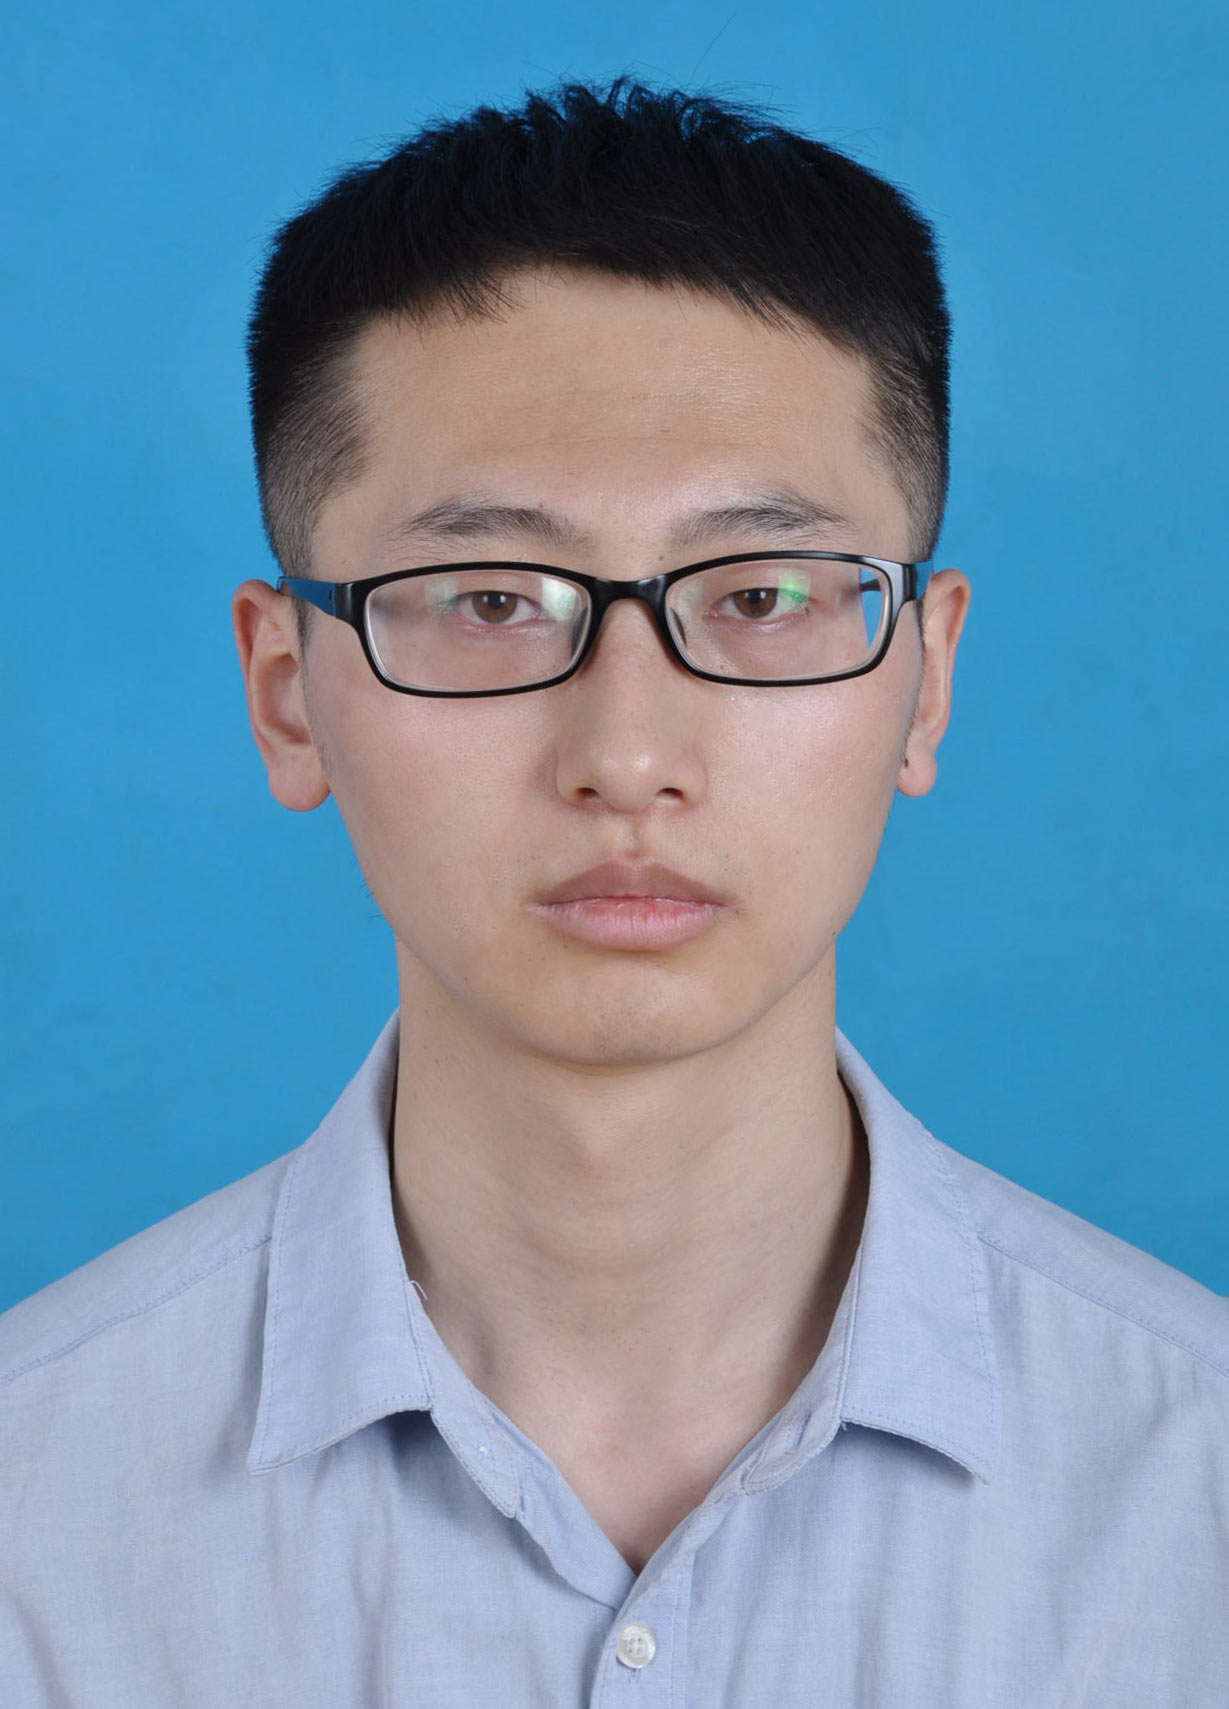
\includegraphics[width=0.88in]{avatar}} &
   \scshape{李高阳} &  \\
    & 性别:男 & 民族:汉 \\
    & 电话:(+86) 15682897374 & 生日:1991-09 \\
    & 邮箱:li.gaoyang@foxmail.com & 微信:sandbox\_ligy\\
    % & 地址:甘肃省兰州市天水南路222号 \hspace{40} & %籍贯:甘肃宁县
    & 个人主页:https://github.com/GoldenRaven & 政治面貌:党员
  \end{tabu}
}

\section{教育经历}
% \textbf{兰州大学}
\datedsubsection{\textbf{兰州大学\ 硕博连读与中科院兰州近物所联合培养博士}}{2013 -- 2019}
\textit{专业:理论物理}\\
\textit{方向:强关联量子系统的数值重整化群研究}
\datedsubsection{\textbf{兰州大学\ 本科}}{2009 --  2013}
\textit{专业:物理学国家基地班\ \ 理论物理}

\section{发表文章}
\textbf{Gao-Yang Li}, Tie-Feng Fang, Ai-Min Guo, and Qing-Feng Sun \textit{Ferromagnetism-induced Kondo effect in graphene with a magnetic impurity}, Phys. Rev. B \textbf{100}, 115115 (2019).

\section{获奖情况}
\datedline{\textit{国家励志奖学金}}{2010 -- 2011}
\datedline{\textit{学校三等奖学金}}{2013 -- 2018}
% \datedline{其他奖项}{2015}

\section{项目经验}
\begin{itemize}%[parsep=0.5ex]
\item \datedline{\textbf{{基于C++实现了全密度矩阵数值重整化群算法}}}{\textbf{{2015/10 -- 2016/08}}}
{\textbf{项目描述}:我们需要数值求解量子杂质问题,而“全密度矩阵数值重整化群算法”是近年来对传统数值重整化群算法的新发展,是计算量子杂质问题最准确最稳定的算法之一。该算法利用迭代的形式实现了重整化,最后得到整个系统的有限本征态与本征值。其中涉及自洽迭代、消除累积误差、矩阵乘法、稠密矩阵对⻆化等矩阵向量操作。实现中调用了 Intel MKL 库,并作了单节点 OpenMP 并行优化。该程序已可以用来求解一些量子杂质问题,部分研究成果整理成了学术论文,已正式发表。}\\
\textbf{职责描述}:独立完成了算法的调研、公式推导、程序结构的设计、程序的编写及优化,并完成后续对物理问题的探索与总结。
\item
\datedline{\textbf{{基于FORTRAN实现了模拟退火算法}}}{\textbf{{2014/08 -- 2014/10}}}
\textbf{项目描述}:为了研究量子Rabi模型的相变,需要求得基态,即能量最小的本征态。导师基于对物理问题的认识提出了猜测基态波函数,对其态波函数作变分优化即可得到基态,进而研究其相变。 对一个有 8 个自变量的函数最小值优化问题,需要用数值方法在大参数范围内得到其稳定的最小值。\\
\textbf{职责描述}:调研并实现了模拟退火算法,在感兴趣的参数范围内对程序进行了调试,在变分求解 Rabi 模型的应用中达到了较好的阶段性结果。
\end{itemize}

\section{其他技能}
% increase linespacing [parsep=0.5ex]
\begin{itemize}%[parsep=0.5ex]
\item 能高效使用Shell脚本,有六年的Linux使用经验,并熟悉Python等
\item 英语六级467,能流利进行口头交流
% \item 平常编写代码要求尽量高效、美观,并用git管理代码
% \item 自学能力强,对新知识有较高的学习热情,并能投入精力解决问题
% \item 自学了机器学习的基本知识
\item 了解精确对角化、密度矩阵重整化群、蒙特卡罗、张量网络重整化群等数值计算方法
% \item 喜欢打羽毛球
\item 本科学习成绩在全班前30\%
\item 对机器学习感兴趣,正在自学TensorFlow框架
\end{itemize}

\section{自我评价}
\qquad 自认为是一个上进努力有责任心的人,能和周围的人和睦相处,进行高效的交流。自学能力强,对新知识有较高的学习热情,能够自驱地学习需要的知识,并能投入精力解决问题。

% \section{个人主页}
% \rm{https://github.com/GoldenRaven}

%% Reference
% \newpage
% \bibliographystyle{IEEETran} \bibliography{mycite}
\end{document}
